\chapter{Prácticas}

Recordemos que todas las contraseñas van a ser \textbf{ABD3oradba}. El usuario que se va a usar como principal durante todo el desarrllo de la parte práctica es \textit{oracle}.

\textbf{Arrancar la base de datos}

\begin{lstlisting}[ language=bash,
                    deletekeywords={IDENTITY},
                    deletekeywords={[2]INT},
                    morekeywords={clustered},
                    framesep=8pt,
                    xleftmargin=40pt,
                    framexleftmargin=40pt,
                    frame=tb,
                    framerule=0pt ]
# arrancar el listener
lsnrctl start
# activar el shell de SQL
sqlplus /nolog
# nos conectamos como administrador
connect sys as sysdba
# levantar la BD
startup
\end{lstlisting}

Para consultar una interfaz gráfica puedes navegar a una de las siguientes direcciones:

\begin{itemize}
\item https://pclab.localdomain:5500/em
\item https://localhost:5500/em
\end{itemize}

\textbf{Detener la base de datos}

\begin{lstlisting}[ language=bash,
                    deletekeywords={IDENTITY},
                    deletekeywords={[2]INT},
                    morekeywords={clustered},
                    framesep=8pt,
                    xleftmargin=40pt,
                    framexleftmargin=40pt,
                    frame=tb,
                    framerule=0pt ]
# acceder al shell de SQL
sqlplus sys as sysdba
# derribar la BD
shutdown immediate
# parar el listener
lsnrctl stop
\end{lstlisting}

\section{Componentes de la arquitectura Oracle}

A groso modo, tenemos los usuarios, una aplicación o servidor red y el servidor donde se ejecuta Oracle. Cuando un usuario quiere conectarse a nuestra base de datos, lo hace a través del listener, que crea un proceso en el servidor para atender nuestras consultas. El usuario hace esto a través del \textbf{proceso de usuario} (que es la aplicación que se conecta a la BD). Esta aplicación puede ser o \textit{SQL*Plus}, Oracle Enterprise Manager, etc, e incluya la Interfaz de Programa de Usuario (UPI). Este proceso genera llamadas al servidor Oracle.

El \textbf{proceso del servidor} se ejecut en la máquina que hostea el servidor Oracle. Sirve a un sólo proceso de usuario si está configurado en modo de \textit{servidor dedicado}. Es importante recordar que este proceso usa una \textbf{Program Global Area (PGA)} exclusiva, que no es más que una zona \textit{privada} de memoria que contiene la información relativa a este proceso. Además incluye la \textbf{Interfaz de Programa de Oracle (OPI)} (que no sé lo que es porque en google no me sale). Este proceso es el encargado de procesar las llamadas generadas por el cliente y de devolverle los resultados.

\begin{figure}[H]
  \center
  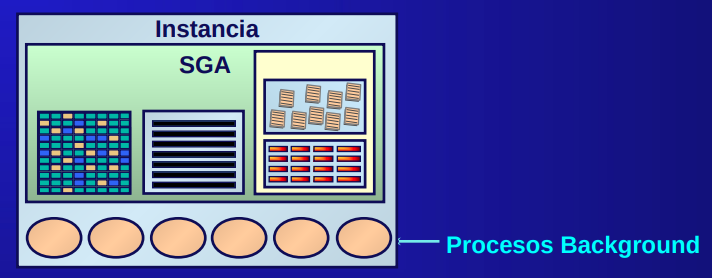
\includegraphics[scale=0.3]{img/p1.png}
\end{figure}

Una instancia está compuesta por la \textbf{System Global Area} y varios procesos background. El SGA es una estructura básica de memoria de Oracle que sirve para facilitar la transferencia de información entre usuarios y también almacena la información estructural de la base de datos más frecuentemente requerida. La memoria necesaria para esta área es automáticamente reservada por Oracle al levantar una instancia de la BD. A su vez el SGA está formado por varios componentes que veremos en la siguiente sección.

\begin{figure}[H]
  \center
  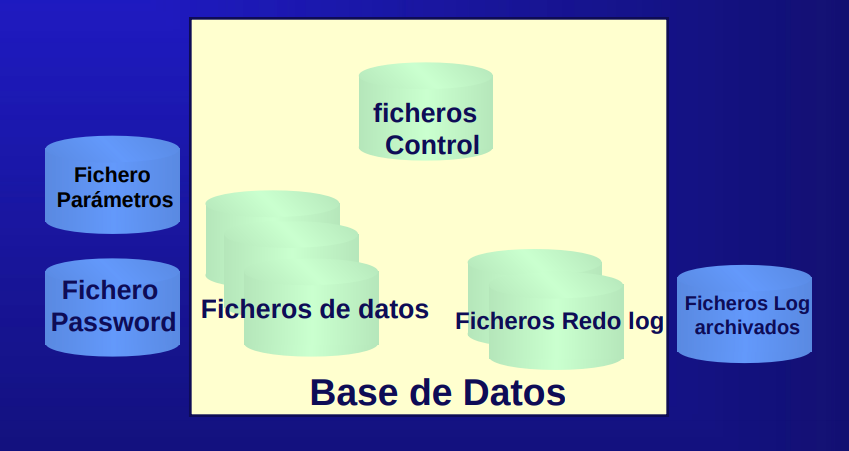
\includegraphics[scale=0.3]{img/p2.png}
\end{figure}

La base de datos está formada por muchos ficheros diferentes. Parte de esos archivos están fuera de la base de datos porque es necesario consultarlos antes de levantar una instancia. Por ejemplo, los \textit{ficheros de password}, que te dicen que usuarios tienen permisos. A esos archivos sólo pueden acceder el administrador y a lo sumo el mismo usuario.

El \textbf{fichero de parámetros} tiene dos modos: texto y binario. Antes de ser modificado, se pasa de binario a texto, se modifica, y se vuelve a almacenar en binario. Es el primer fichero consultado por la instancia y contiene donde se encuentran los archivos de la base de datos, los ficheros que la componen, el modo en el que va a funcionar, etc. Sólo contiene la información básica para que pueda arrancar. El administrador tiene como tarea hacer backups de este fichero de forma regular. Los \textbf{ficheros redo log} contienen copias de los bloques sucios.

Al levantar la instancia, los ficheros consultados son:
\begin{itemize}
\item Fichero password
\item Fichero parámetros
\item Ficheros control
\end{itemize}

Para interactuar con la base de datos, es necesario levantarla, y después, levantar también un listener, que es nuestro medio de comunicación con la BD. Una vez levantado, para poder hacer cosas tenemos que ejecutar el software necesario de Oracle. Por ejemplo, si usamos SQLPlus (nuestro proceso de usuario), éste se conecta con el listener y éste a su vez con la BD. 

Lo más común es levantar la BD en \textit{modo dedicado}, es decir, cada petición que le llega al listener es atendida por un proceso especialmente creado para esa consulta.

\subsection{Shared Pool}

\begin{figure}[H]
  \center
  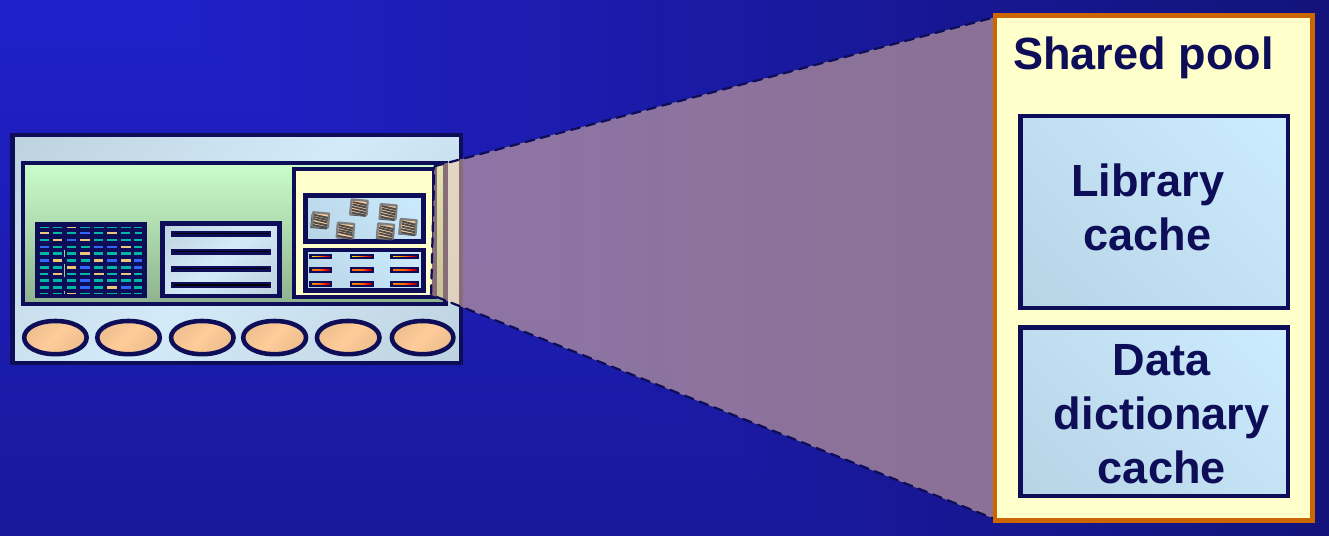
\includegraphics[scale=0.2]{img/p3.png}
\end{figure}

Este componente puede ser dividido en dos grandes secciones: la \textbf{library cache} y la \textbf{dictionary cache}. Veámoslos:
\begin{itemize}
\item Library cache: está diseñada para incrementar la eficiencia del código SQL permitiendo que se compartan entre los usuarios las sentencias tanto SQL como PL/SQL. Aquí se almacenan todas las sentencias SQL parseadas. 

Cuando un usuario ejecuta una sentencia ocurren dos cosas. Primero Oracle verifica si ya existe en la libary cache una sentencia idéntica. Si no se encuentra, la sentencia debe ser parseada y luego alojada en la library cache. Si existiera, se reutiliza el resultado del parseo hehco en su momento.

\item (Data) dictionary cache: el objetivo de este componente es reducir los accesos a disco. Es similarr a la library cache en el sentido de que ambas mantienen información reciente en memoria. El catálogo contiene metadatos de la misma BD, y la dictionary cache se encarga de cacheare esos metadatos. Si Oracle necesita alguno de esos datos, los busca primero aquí y si no los encuentra consulta el catálogo.
\end{itemize}

El tamaño de este componente puede ser configurado usando \textit{SHARED\_POOL\_SIZE}.

\subsection{Buffer Cache de la BD}

\begin{figure}[H]
  \center
  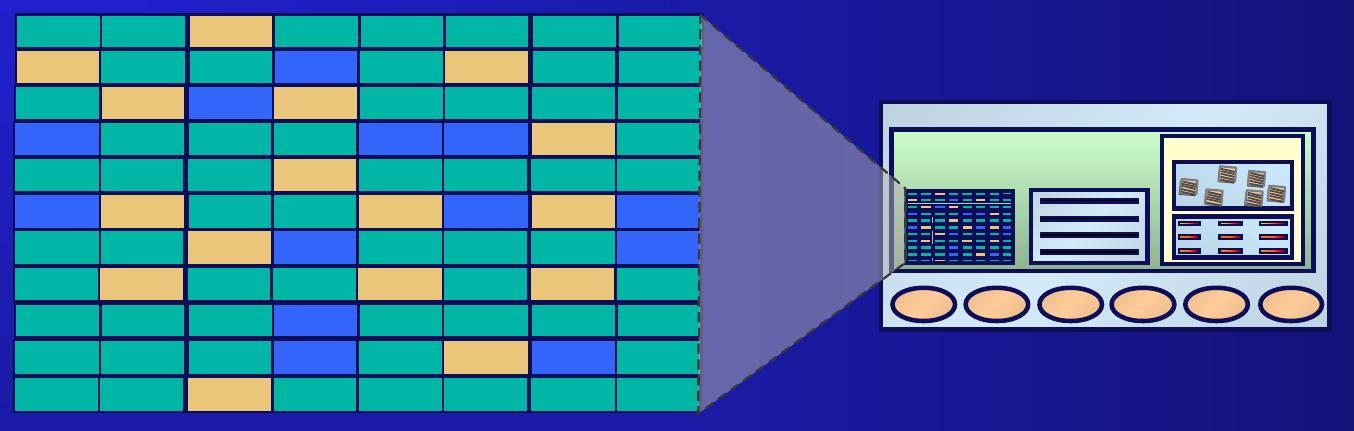
\includegraphics[scale=0.2]{img/p4.png}
\end{figure}

El \textbf{buffer cache} almacena copias de los \textit{bloques de datos} en memoria. Normalmente, por eficiencia, el tamaño de este buffer es múltiplo del tamaño del bloque de datos. Este buffer está compartido entre todas las sesiones conectadas a la BD. La finalidad principal es mantener los bloques de usados más frecuentemente usados en memoria para mejorar la eficiencia (reduciendo los accesos a disco). Cuando un bloque sucio (ocupado) deja de ser usado, es escrito a disco por el \textit{Database Writer background process}.

La cantidad de buffers puede ser definida usando \textit{DB\_BLOCK\_BUFFERS}. El tamaño del buffer está basado en el parámetro \textit{DB\_BLOCK\_SIZE}.

\subsection{Porgram Global Area (PGA)}

\begin{figure}[H]
  \center
  
\includegraphics[scale=0.2]{img/p5.png}
\end{figure}

Es una zona de memoria que contiene datos e información de control para un \textit{Proceso de Servidor}. Esta memoria no es compartida con nadie (excepto el proceso en sí). Es creada por Oracle cuando el proceso arranca. Hay una zona PGA por \textit{cada} proceso de servidor. Los \textbf{background processes} también crean sus propios PGAs.

\subsection{Buffer Redo Log}

\begin{figure}[H]
  \center
  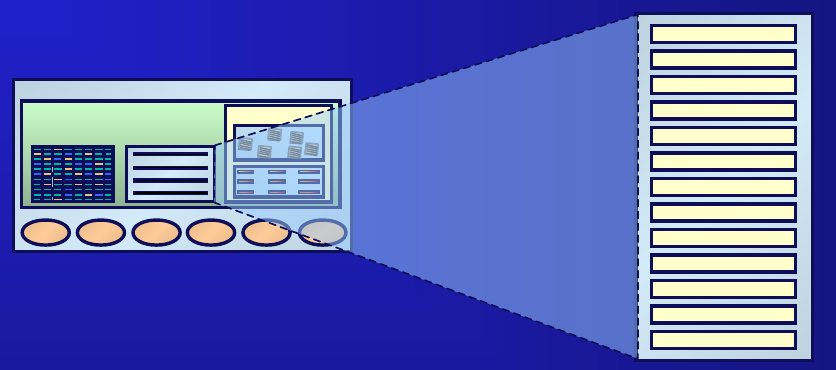
\includegraphics[scale=0.2]{img/p6.png}
\end{figure}

En este área de memoria se almacena información sobre los cambios a la BD, llamados \textit{entradas redo log}. Estas entradas son usadas si la recuperación de la base de datos es necesario (rollback). Contienen la información necesaria para reconstruir los cambios hechos por alguna de las siguientes sentencias: \textit{INSERT}, \textit{UPDATE}, \textit{DELETE}, \textit{CREATE}, \textit{DROP} o \textit{AlTERT}.

Este buffer es circular, es decir, cuando está lleno, las entradas son escritas desde el principio. El proceso LGWR escribe los contenidos de este buffer al correspondiente archivo redo log en disco. El tamaño de este buffer puede ser especificado en el parámetro \textit{LOG\_BUFFER}.


\subsection{Database Writer (DBWR)}

\begin{figure}[H]
  \center
  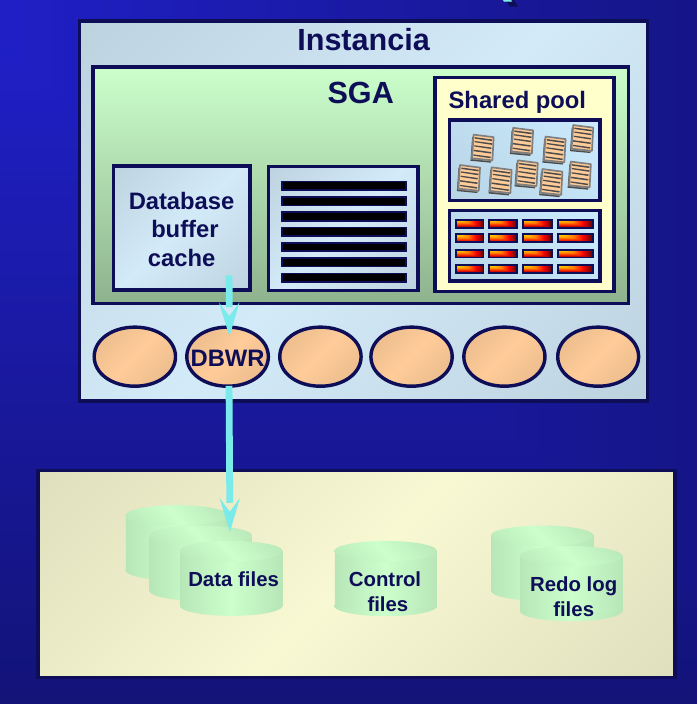
\includegraphics[scale=0.2]{img/p7.png}
\end{figure}

Este proceso es el encargado de escribir los bloques de datos del buffer cache a archivos de datos (\textit{data files}). Los bloques de datos no son inmediatamente escritos a un datafile, los bloques son acumulados para posteriormente escribirlos de golpe en su correspondientes datafiles. Importante, la escritura a disco puede pasar antes o después de hacer un \textit{commit}. Después del commit, la BD escribe seguro los redo buffers en disco, pero no los bloques de datos.

\subsection{Log Writer (LGWR)}

\begin{figure}[H]
  \center
  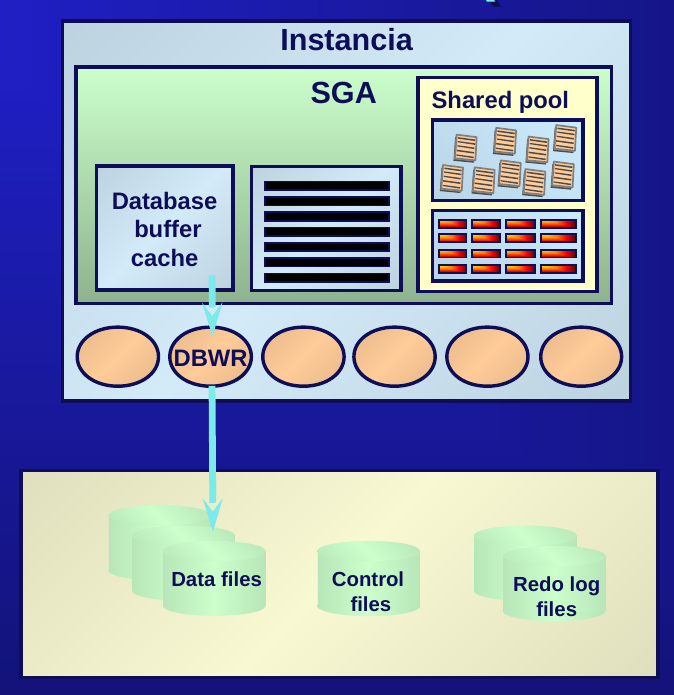
\includegraphics[scale=0.2]{img/p9.png}
\end{figure}

Es el responsable de la administración de la escritura del buffer redo log (en memoria) a un determinado archivo redo log (en disco). Como el buffer redo log es un buffer circular, sólamente  se pueden escribir nuevas entradas cuando el LGWR ha escrito las que antes había a disco. Normalmente, el LGWR es suficientemente rápido para asegurar que siempre hay espacio disponible para escribir nuevas entradas.

\subsection{Procesamiento de un commit}

\begin{figure}[H]
  \center
  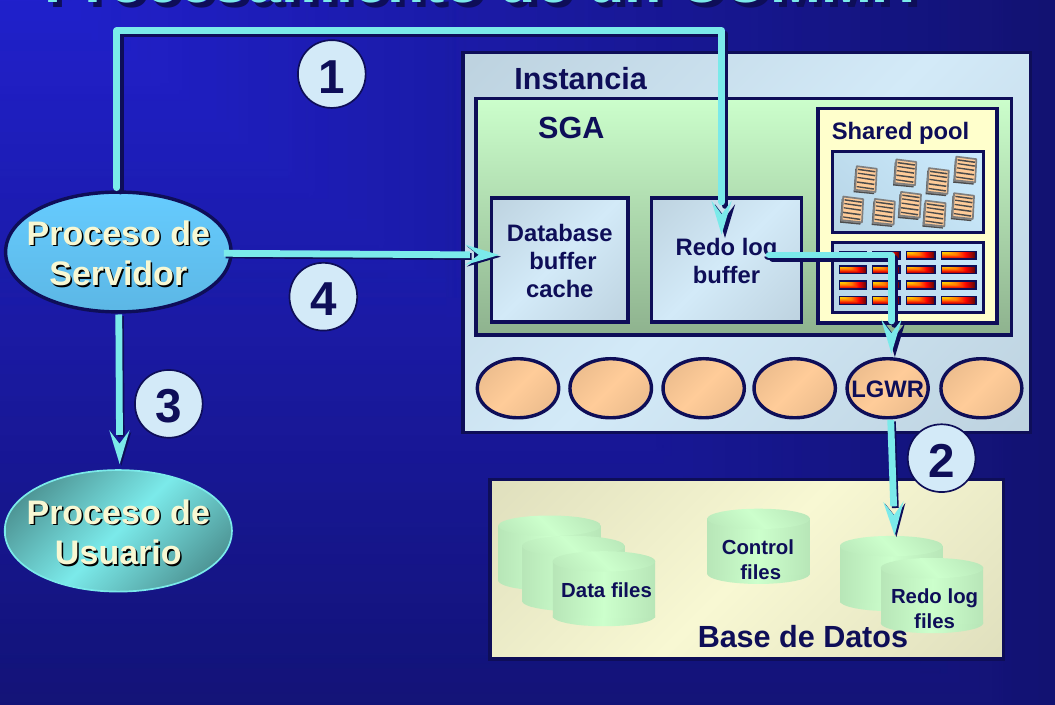
\includegraphics[scale=0.2]{img/p8.png}
\end{figure}

La sentencia \textit{COMMIT} es usada para terminar tu transacción actual y hacer permanentes los cambios llevadas a cabos por ella. Una \textit{transacción} es una sequencia de sentencias SQL que Oracle trata como un única unidad. Esta sentencia también borra todos los puntos de guardado en la transacción y levanta los bloqueos hechos por la transacción. Antes de hacer \textit{COMMIT}, tu puedes ver los datos afectados por tu transacción, pero no otros usuarios que accedan a esos mismos datos.  

Pasos de la fotografía:
\begin{enumerate}
\item El proceso de servidor recibe la consulta y escribe las entradas necesarias en el buffer redo log.
\item El proceso LGWR escribe las entradas redo log que queden pendientes a disco. Este punto se considera el final de la transacción \textit{commit}.
\item Oracle desbloquea los cerrojos necesarios por la transacción y permite a los usuarios esperando continuar con su trabajoo.
\item Si se detectan bloques que ya no van a ser usados, se pasan a disco.
\end{enumerate}

Es importante tener en mente que Oracle siempre ejecuta un \textit{COMMIT} antes y después de ejecutar cualquier sentencia perteneciente al DDL (\textit{Data Definition Language}).

Para tener una imagen más o menos simple de todo lo que hemos visto de Oracle en esta sección:

\begin{figure}[H]
  \center
  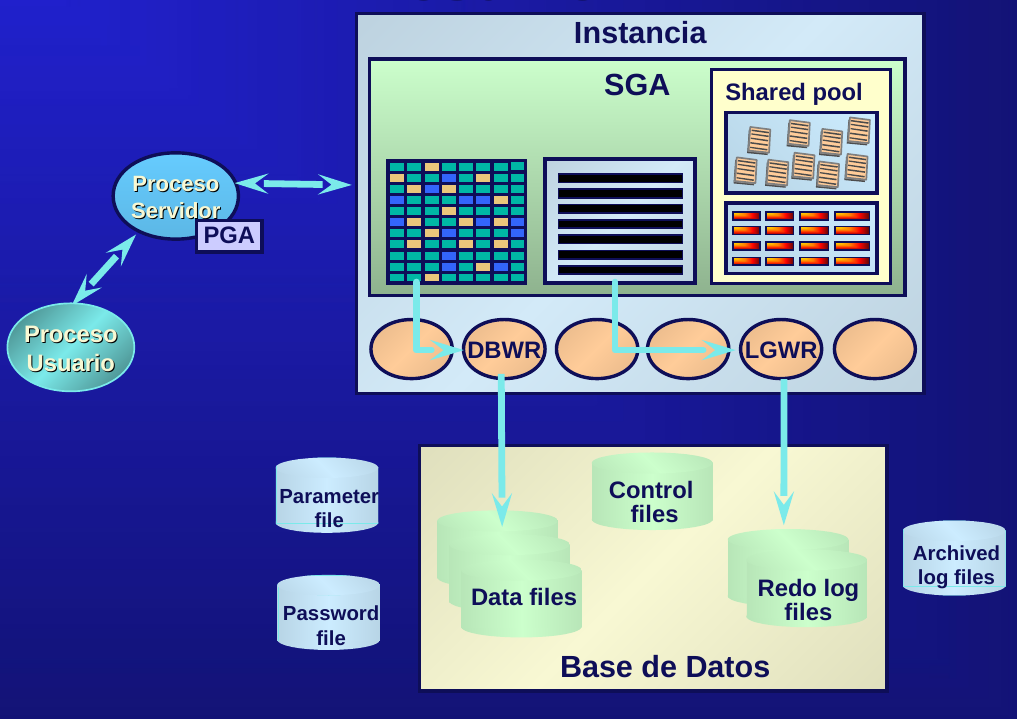
\includegraphics[scale=0.3]{img/p11.png}
\end{figure}

\section{Gestión de Red}

Obteivos principales de esta sección:
\begin{itemize}
\item Conocer el procedimiento mediante el cual Net establece una conexión con un servidor.
\item Identificar los componentes fundamentales de la arquitectura Net y como interactúan.
\end{itemize}

\subsection{Conexión a un servidor}

El componente \textit{Net} nos proporciona tres funciones básicas:
\begin{itemize}
\item Operaciones de conexión
\item Operaciones de transporte de datos
\item Operaciones de excepción
\end{itemize}
La arquitectura \textit{Net} se compone de varias capas, cada una de ellas tiene un único cometido en una sesión de red.

El \textit{Oracle Net Listener} es un proceso separado que se ejecuta en el servidor donde está la BD. Recibe las peticiones entrantes de los clientes y administra el tráfico de estas peticiones al servidor de la BD. 

\underline{\textbf{Conexión al servidor}}

\begin{figure}[H]
  \center
  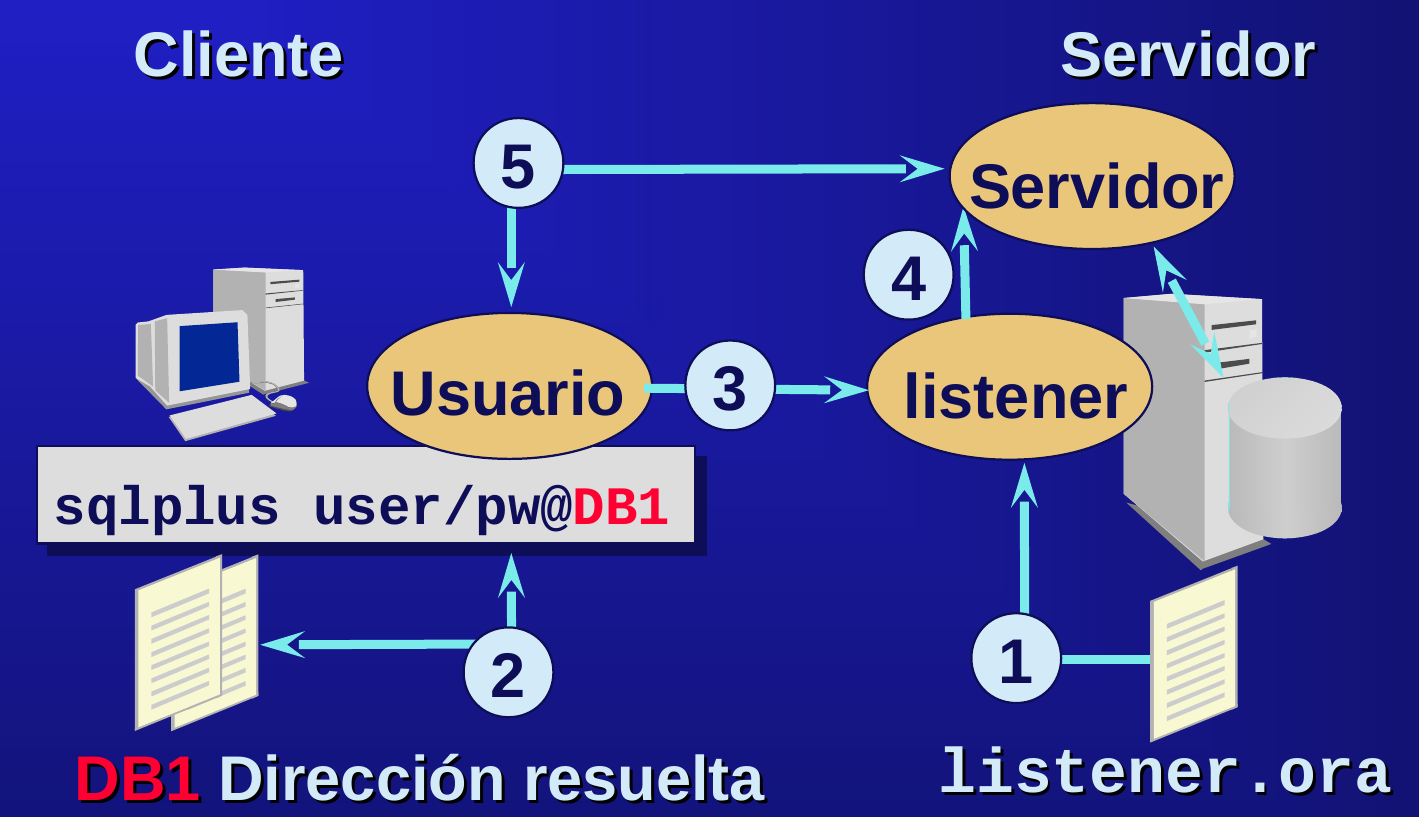
\includegraphics[scale=0.2]{img/p12.png}
\end{figure}

Para conectarnos desde el cliente a la BD, podemos usar la sentencia:

\begin{lstlisting}[ language=SQL,
                    deletekeywords={IDENTITY},
                    deletekeywords={[2]INT},
                    morekeywords={clustered},
                    framesep=8pt,
                    xleftmargin=40pt,
                    framexleftmargin=40pt,
                    frame=tb,
                    framerule=0pt ]
sqlplus user/pw@DB1
\end{lstlisting}
Donde \textit{user} es nuestro usuario y \textit{DB1} es la dirección IP del servidor alojando la BD. Estos parámetros pueden ser específicados por defecto usando: 
\begin{itemize}
\item \textit{tsnames.ora}: es un archivo de configuración que contiene nombres de servicios en red mapeados,asignados a ddescriptores a través de los cuáles se nos permite acceder. Está ubicado en los clientes. Algunos parámetros del archivo son:
\begin{itemize}
\item HOST: dirección ip del servidor con el que nos queremos conectar.
\item PORT: puerto donde escucha la base de datos.
\item SERVICE\_NAME: nombre del servicio de la base de datos al que queremos conectarnos.
\end{itemize}
\item \textit{sqlnet.ora}: es un archivo de texto que proporciona al cliente la información básica sobre la red (como el dominio por defecto, encriptación, etc). Este fichero también se encuentra únicamente en el cliente.
\item \textit{listener.ora}: aquí se encuentran los parámetros de configuración del listener. Tiene un formato en modo texto pero es muy recomendable modificarlo solo a través de la GUI de Oracle Enterprise Manager. Este fichero se encuentra solo en el servidor. Algunos de sus parámetros son:
\begin{itemize}
\item \textit{LISTENER}: nombre del listener.
\item \textit{SID}: nombre de la BD por defecto.
\item \textit{ADDRESS}: 
  \begin{itemize}
    \item \textit{PROTOCOL}: protocolo usado para la comunicación.
    \item \textit{HOST}: nombre del host.
    \item \textit{PORT}: puerto donde escuchará el listener.
  \end{itemize}
\end{itemize}
\end{itemize}
Estos ficheros pueden ser encontrados en $\$ORACLE\_HOME/network/admin$

\underline{\textbf{Desconexión de un servidor}}

Puede ser decidida por el usuario (voluntariamente). El servidor puede producirla si se ha superado un determinado tiempo. O también puede ocurrir por causas anómalas (caíde de red, etc).

\underline{\textbf{Protocolo Bequeath}}

Cuando un cliente hace una petición de conexión a un servidor, el listener creará un proceso de servidor y legará la conexión a ese, o redireccionará la conexión a un proceso de servidor existente.

El protocolo o secuencia \textit{Bequeath} permite a los clientes conectarse a la base de datos sin usar el listener. Internamente, este protocolo levanta un proceso de servidor para cada aplicación cliente. Hace exactamente lo mismo que el listener hace para una conexión local. Este protocolo sólo es usado para conexiones locales donde una alicación cliente (como \textit{SQLPlus}), se comunica con la instancia de la base de datos corriendo en el mismo ordenador. Sólo funcione si el servidor está en modo dedicado (cada petición un proceso de servidor).

Aquí faltaría hablar un poco de la sesión redireccionada, que hay dos casos: la dedicada y la dispatcher.

\subsection{Utilidad lsnrctl}

La utilidad de control del listener es la herramienta para gestionar el listener. Se pueden ejecutar comandos de control desde la línea de comandos o desde el prompt de \textit{lsnrctl}. 
\begin{lstlisting}[ language=bash,
                    deletekeywords={IDENTITY},
                    deletekeywords={[2]INT},
                    morekeywords={clustered},
                    framesep=8pt,
                    xleftmargin=40pt,
                    framexleftmargin=40pt,
                    frame=tb,
                    framerule=0pt ]
lsnrctl <command>
\end{lstlisting}
Las funciones más usadas son las de iniciar y detener el listener:
\begin{lstlisting}[ language=bash,
                    deletekeywords={IDENTITY},
                    deletekeywords={[2]INT},
                    morekeywords={clustered},
                    framesep=8pt,
                    xleftmargin=40pt,
                    framexleftmargin=40pt,
                    frame=tb,
                    framerule=0pt ]
lsnrctl start
lsnrctl stop
\end{lstlisting}
El modificador \textit{SET} se usa para cambiar parámetros del listener en el entorno del \textit{lsnrctl}:
\begin{lstlisting}[ language=bash,
                    deletekeywords={IDENTITY},
                    deletekeywords={[2]INT},
                    morekeywords={clustered},
                    framesep=8pt,
                    xleftmargin=40pt,
                    framexleftmargin=40pt,
                    frame=tb,
                    framerule=0pt ]
LSNRCTL> SET trc_level ADMIN
\end{lstlisting}
El modificador \textit{SHOW} se usa para visualizar los valores de los parámetros para el listener:
\begin{lstlisting}[ language=bash,
                    deletekeywords={IDENTITY},
                    deletekeywords={[2]INT},
                    morekeywords={clustered},
                    framesep=8pt,
                    xleftmargin=40pt,
                    framexleftmargin=40pt,
                    frame=tb,
                    framerule=0pt ]
LSNRCTL> SHOW connect_timeout
\end{lstlisting}

\subsection{Configuración del lado del cliente}

Vamos a establecer una conexión del lado del cliente de Net usando el método \textit{host naming}. Este método no precisa de configuración, a diferencia del \textit{local naming}, que es necesario configurarlo usando la herramiento gráfica \textit{Net manager}.

Esto tengo que completarlo.

\section{Manejo de una instancia Oracle}

Una instancia de Oracle presenta la siguiente estructura: 

\begin{figure}[H]
  \center
  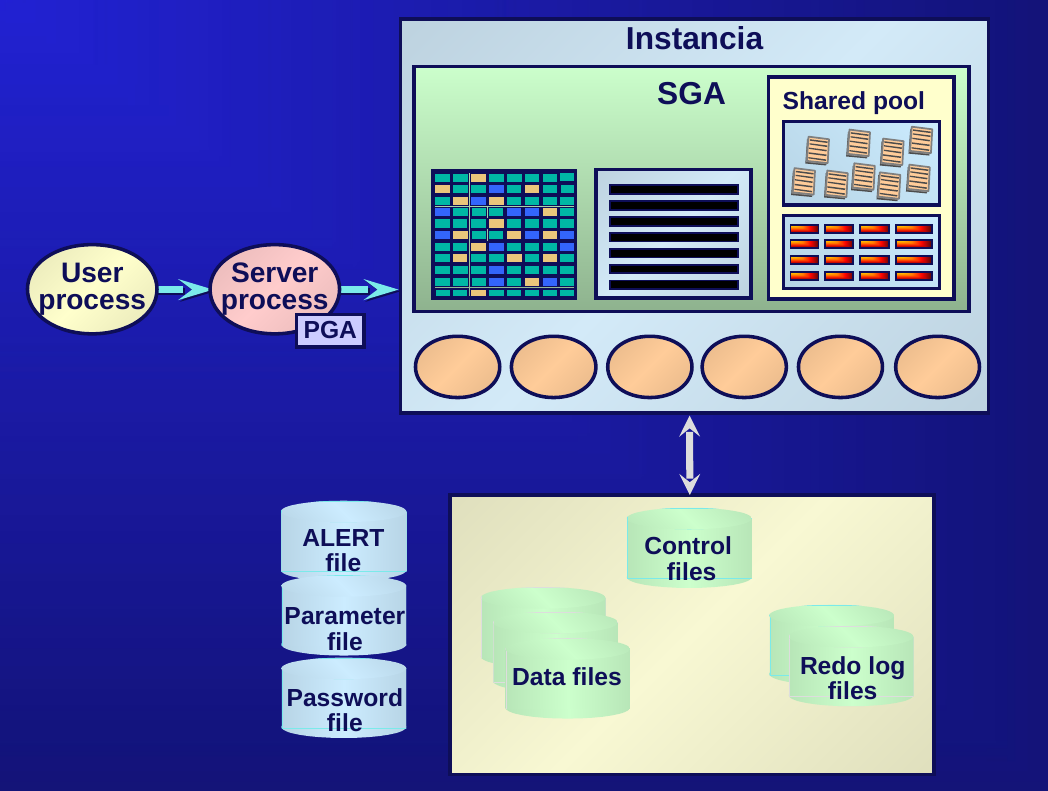
\includegraphics[scale=0.3]{img/p13.png}
\end{figure}

En la BD hay dos usuarios administradores \textbf{SYS} y \textbf{SYSTEM}. Son creados automáticamente y se les asigna el rol \textbf{SYSDBA}.
\begin{itemize}
\item \underline{SYS}: Su contraseña es asignada durante el proceso de instalación de la BD. Es el propietario de los datos del diccionario de la BD.
\item \underline{SYSTEM}: Su contraseña es asignada durante el proceso de instalación de la BD. Propietario de tablas internas adicionales usadas por Herramientas Oracle.
\end{itemize}

Hay diferentes métodos de autenticación, a través del fichero \textit{password} o a través del SO:

\begin{figure}[H]
  \center
  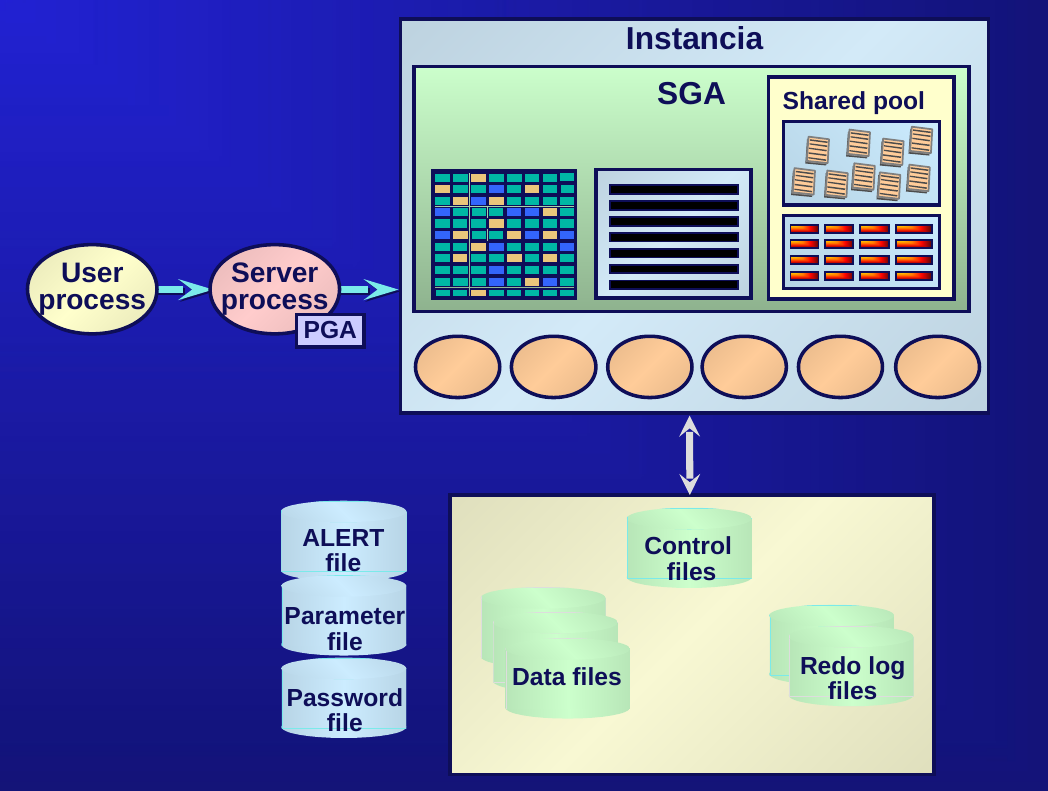
\includegraphics[scale=0.3]{img/p13.png}
\end{figure}

Para crear el fichero de \textit{password} usando la utilidad de \textit{password}, se usa el siguiente comando:
\begin{lstlisting}[ language=bash,
                    deletekeywords={IDENTITY},
                    deletekeywords={[2]INT},
                    morekeywords={clustered},
                    framesep=8pt,
                    xleftmargin=40pt,
                    framexleftmargin=40pt,
                    frame=tb,
                    framerule=0pt ]
$ orapwd file=$ORACLE_HOME/dbs/orapworadba entries=5
\end{lstlisting}

Para decirle a la instancia si usar un fichero \textit{password} o no, se usa el parámetro \textit{REMOTE\_LOGIN\_PASSWORDFILE}. El valor de este parámetro se especifica durante el proceso de instlación de la base de dtos. Tiene 3 valores distintos:
\begin{itemize}
\item \textit{shared}: una o varias bases de datos pueden usar el archivo \textit{password}.
\item \textit{exclusive}: el archivo solo puede ser usado por una base de datos.
\item \textit{none}: el archivo \textit{password} es ignorado completamente, luego los usuarios se deben autenticar usando el sistema operativo.
\end{itemize}
Para conectarse a la base de datos:
\begin{lstlisting}[ language=bash,
                    deletekeywords={IDENTITY},
                    deletekeywords={[2]INT},
                    morekeywords={clustered},
                    framesep=8pt,
                    xleftmargin=40pt,
                    framexleftmargin=40pt,
                    frame=tb,
                    framerule=0pt ]
CONNECT sys/ABD3oradba as sysdba
\end{lstlisting}

\subsection{Fichero de parámetros del servidor, SPFILE}

El archivo \textit{SPFILE} no se puede modificar directamente porque puede producir graves inconsistencias. Para modificarlo, hay que obtener un \textit{PFILE} a partir del \textit{SPFILE} actual:
\begin{lstlisting}[ language=bash,
                    deletekeywords={IDENTITY},
                    deletekeywords={[2]INT},
                    morekeywords={clustered},
                    framesep=8pt,
                    xleftmargin=40pt,
                    framexleftmargin=40pt,
                    frame=tb,
                    framerule=0pt ]
CREATE PFILE="/databases/app/oracle/admin/oradba/pfile/init.ora" FROM SPFILE="/databases/app/oracle/product/12.2.0.1/db_1/dbs/spfileoradba.ora";
\end{lstlisting}
Una vez creado este archivo, se cambian los atributos que se quieran y se guarda el archivo. Ahora hay que detener la instancia y arrancarla con el nuevo \textit{PFILE}. Si se ha terminado de modificar el archivo, se crea un nuevo \textit{SPFILE} a partir de ese archivo y se inicia la BD de nuevo (sin usar la cláusula \textit{PFILE}).
\begin{lstlisting}[ language=bash,
                    deletekeywords={IDENTITY},
                    deletekeywords={[2]INT},
                    morekeywords={clustered},
                    framesep=8pt,
                    xleftmargin=40pt,
                    framexleftmargin=40pt,
                    frame=tb,
                    framerule=0pt ]
SHUTDOWN IMMEDIATE;
STARTUP;
\end{lstlisting}
Muchos de los parámetros de la BD se pueden almacenar directamente en la base de datos, por esa razón el \textit{SPFILE} solo incluye los parámetros necesarios para iniciar la instancia. Esto facilita el cambio dinámico de parámetros de la instancia. El primer \textit{SPFILE} es creado automáticamente a partir de los parámetros proporcionados en el Asistente de Instalación. Se puede crear un \textit{SPFILE} con el siguiente comando:
\begin{lstlisting}[ language=bash,
                    deletekeywords={IDENTITY},
                    deletekeywords={[2]INT},
                    morekeywords={clustered},
                    framesep=8pt,
                    xleftmargin=40pt,
                    framexleftmargin=40pt,
                    frame=tb,
                    framerule=0pt ]
CREATE SPFILE="/databases/app/oracle/product/12.2.0.1/db_1/dbs/spfileoradba.ora" FROM PFILE="/databases/app/oracle/admin/oradba/pfile/copia_init.ora";
\end{lstlisting}

Para iniciar una instancia usando el fichero \textit{PFILE}:

\begin{lstlisting}[ language=SQL,
                    deletekeywords={IDENTITY},
                    deletekeywords={[2]INT},
                    morekeywords={clustered},
                    framesep=8pt,
                    xleftmargin=40pt,
                    framexleftmargin=40pt,
                    frame=tb,
                    framerule=0pt ]
STARTUP PFILE="/databases/app/oracle/admin/oradba/pfile/init.ora";
\end{lstlisting}

Para iniciarla usando el \textit{SPFILE}:
\begin{lstlisting}[ language=SQL,
                    deletekeywords={IDENTITY},
                    deletekeywords={[2]INT},
                    morekeywords={clustered},
                    framesep=8pt,
                    xleftmargin=40pt,
                    framexleftmargin=40pt,
                    frame=tb,
                    framerule=0pt ]
STARTUP;
\end{lstlisting}

\subsection{Fases del inicio y la detención}

\begin{figure}[H]
  \center
  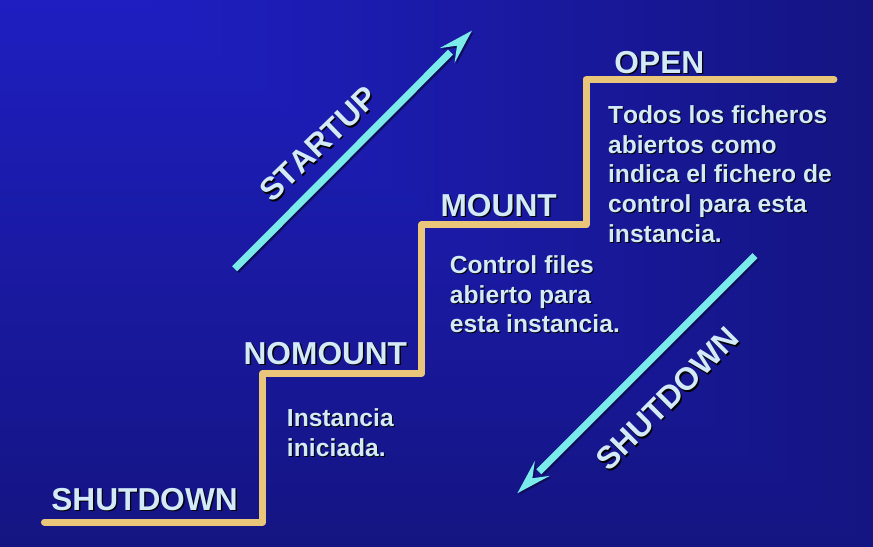
\includegraphics[scale=0.3]{img/p15.png}
\end{figure}

\subsection{Opciones de shutdown}

\begin{tabular}{|c|c|c|c|c|}
\hline 
Modo shutdown & Abort & Immediate & Transactional & Normal \\ 
\hline 
Permite nuevas conexiones & \texttimes & \texttimes & \texttimes & \texttimes \\ 
\hline 
Espera a que termine las conexiones actuales & \texttimes & \texttimes & \texttimes & \checkmark \\ 
\hline 
Espera a que terminen las transacciones actuales & \texttimes & \texttimes & \checkmark & \checkmark \\ 
\hline 
Fuerza un checkpoint y cierra ficheros & \texttimes & \checkmark & \checkmark & \checkmark \\ 
\hline 
\end{tabular}

Dependiendo de que opción se use para apagar la instancia tardará más o menos tiempo. La más rápida es abort y la más lenta el apagado normal.

\subsection{Vistas dinámicas de rendimiento}

Son vistas mantenidas por el servidor Oracle y son constantemente actualizadas. Contienen datos sobre estructuras de disco y memoria, además de datos útiles para el ajuste del rendimiento. Tienen sinónimos públicos con el prefijo $V\$$.

Dependiendo del estado en el que esté la instancia, las vistas dinámicas cambian:

\begin{figure}[H]
  \center
  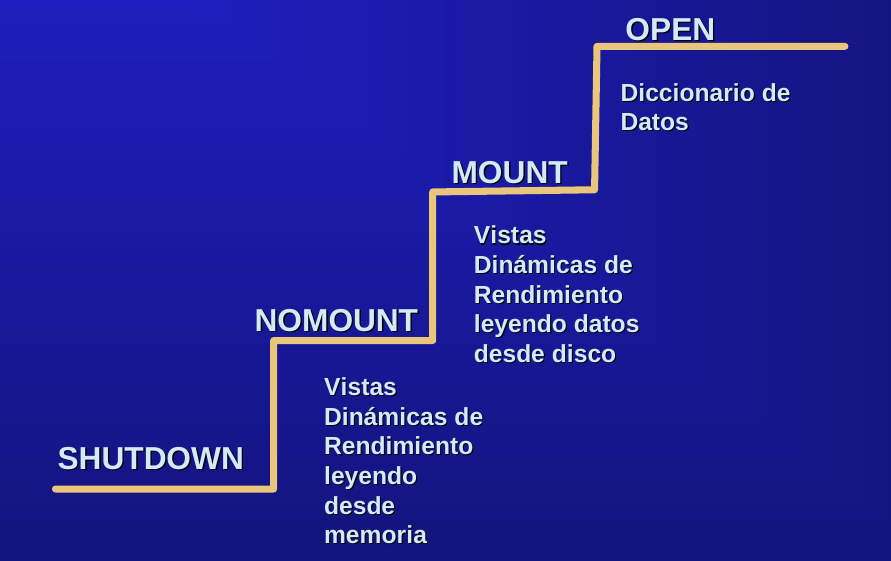
\includegraphics[scale=0.25]{img/p16.png}
\end{figure}

\begin{center}
\begin{tabular}{|c|c|}
\hline 
Se consulta en & Parámetro \\ 
\hline 
 \multirow{7}{*}{SGA} & V\$PARAMETER \\ 
  & V\$SGA \\ 
  & V\$OPTION \\ 
  & V\$PROCESS \\ 
  & V\$SESSION \\ 
  & V\$VERSION \\ 
  & V\$INSTANCE \\ 
\hline 
\multirow{6}{*}{Control file}& V\$THREAD \\ 
  & V\$CONTROLFILE \\ 
  & V\$DATABASE \\ 
  & V\$DATAFILE \\ 
  & V\$DATAFILE\_HEADER \\ 
  & V\$LOGFILE \\ 
\hline 
\end{tabular} 
\end{center}

Para consultar alguno de esos parámetros, se pueden ejecutar consultas como la siguiente:
\begin{lstlisting}[ language=SQL,
                    deletekeywords={IDENTITY},
                    deletekeywords={[2]INT},
                    morekeywords={clustered},
                    framesep=8pt,
                    xleftmargin=40pt,
                    framexleftmargin=40pt,
                    frame=tb,
                    framerule=0pt ]
SELECT name FROM v$parameter WHERE name LIKE "%control%";
\end{lstlisting}
Además, algunos parámetros de inicialización pueden ser modificados mientras la instancia está ejecutándose:
\begin{lstlisting}[ language=SQL,
                    deletekeywords={IDENTITY},
                    deletekeywords={[2]INT},
                    morekeywords={clustered},
                    framesep=8pt,
                    xleftmargin=40pt,
                    framexleftmargin=40pt,
                    frame=tb,
                    framerule=0pt ]
ALTER SESSION SET SQL_TRACE=true;
ALTER SYSTEM SET TIMED_STATISTICS=true;
ALTER SYSTEM SET SORT_AREA_SIZE=131072 DEFERRED;
\end{lstlisting}

\subsection{Manejo de sesiones}

Usar el comando \textit{STARTUP} para restringir el acceso a la base de datos:
\begin{lstlisting}[ language=SQL,
                    deletekeywords={IDENTITY},
                    deletekeywords={[2]INT},
                    morekeywords={clustered},
                    framesep=8pt,
                    xleftmargin=40pt,
                    framexleftmargin=40pt,
                    frame=tb,
                    framerule=0pt ]
STARTUP RESTRICT;
\end{lstlisting}
Usar el comando \textit{ALTER SYSTEM} para poner una instancia en modo restringido:
\begin{lstlisting}[ language=SQL,
                    deletekeywords={IDENTITY},
                    deletekeywords={[2]INT},
                    morekeywords={clustered},
                    framesep=8pt,
                    xleftmargin=40pt,
                    framexleftmargin=40pt,
                    frame=tb,
                    framerule=0pt ]
ALTER SYSTEM ENABLE RESTRICTED SESSION;
\end{lstlisting}
Para finalizar sesiones hay que seguir una serie de pasos:
\begin{enumerate}
\item Identificar la sesión a finalizar con la vista dinámica de rendimiento $v\$session$:
\begin{lstlisting}[ language=SQL,
                    deletekeywords={IDENTITY},
                    deletekeywords={[2]INT},
                    morekeywords={clustered},
                    framesep=8pt,
                    xleftmargin=40pt,
                    framexleftmargin=40pt,
                    frame=tb,
                    framerule=0pt ]
SELECT sid, serial# FROM v$session WHERE username="SYS";
\end{lstlisting}
\item Ejecutar el comando \textit{ALTER SYSTEM}:
\begin{lstlisting}[ language=SQL,
                    deletekeywords={IDENTITY},
                    deletekeywords={[2]INT},
                    morekeywords={clustered},
                    framesep=8pt,
                    xleftmargin=40pt,
                    framexleftmargin=40pt,
                    frame=tb,
                    framerule=0pt ]
ALTER SYSTEM KILL SESSION "7,15";
\end{lstlisting}
\end{enumerate}

\subsection{Ficheros de traza}

Los ficheros de traza pueden ser escritos por el servidor y por los procesos \textit{background}. Oracle vuelca información acerca de errores en los ficheros de traza. El fichero \textit{ALERT} contiene una secuencia cronológica de mensajes y errores. La traza del proceso del servidor se puede habilitar y deshabilitar mediante el comando \textit{ALTER SESSION} o el parámetro \textit{SQL\_TRACE TRUE,FALSE}.
\begin{figure}[H]
  \center
  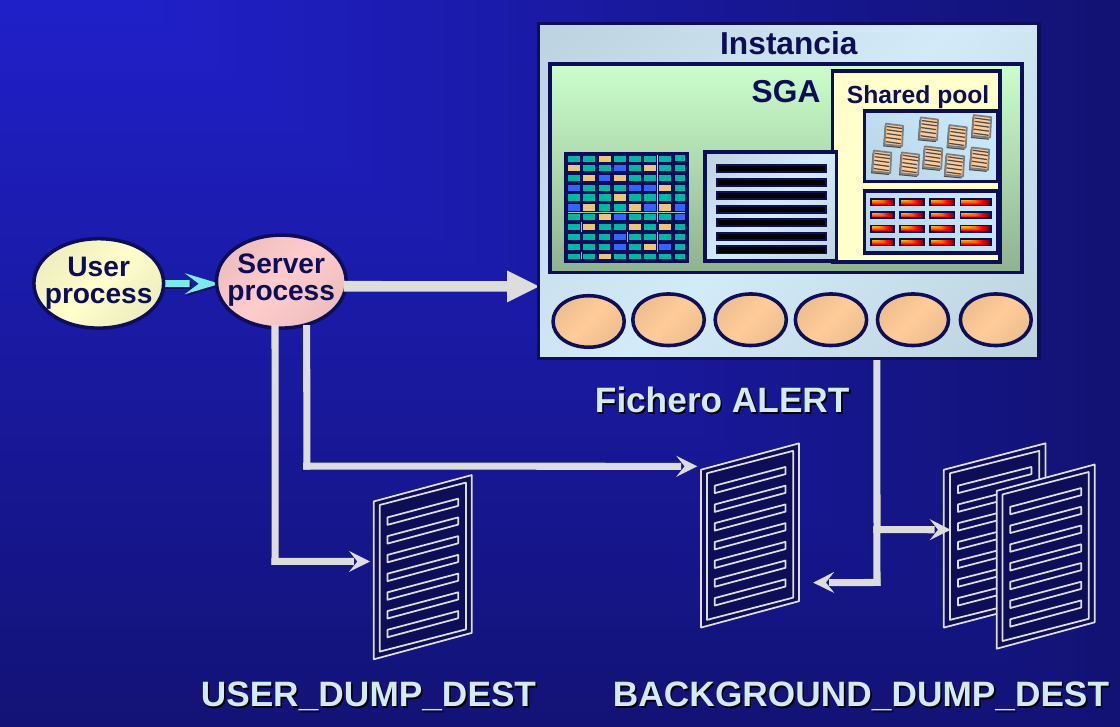
\includegraphics[scale=0.25]{img/p17.png}
\end{figure}
Se recomienda consultar estos ficheros periódicamente para detectar errores internos y errores de corrupción, monitorizar operaciones sobre la base de datos y visualiar los parámetros de inicialización no establecidos por defecto.

\section{Creación de una base de datos}

\begin{figure}[H]
  \center
  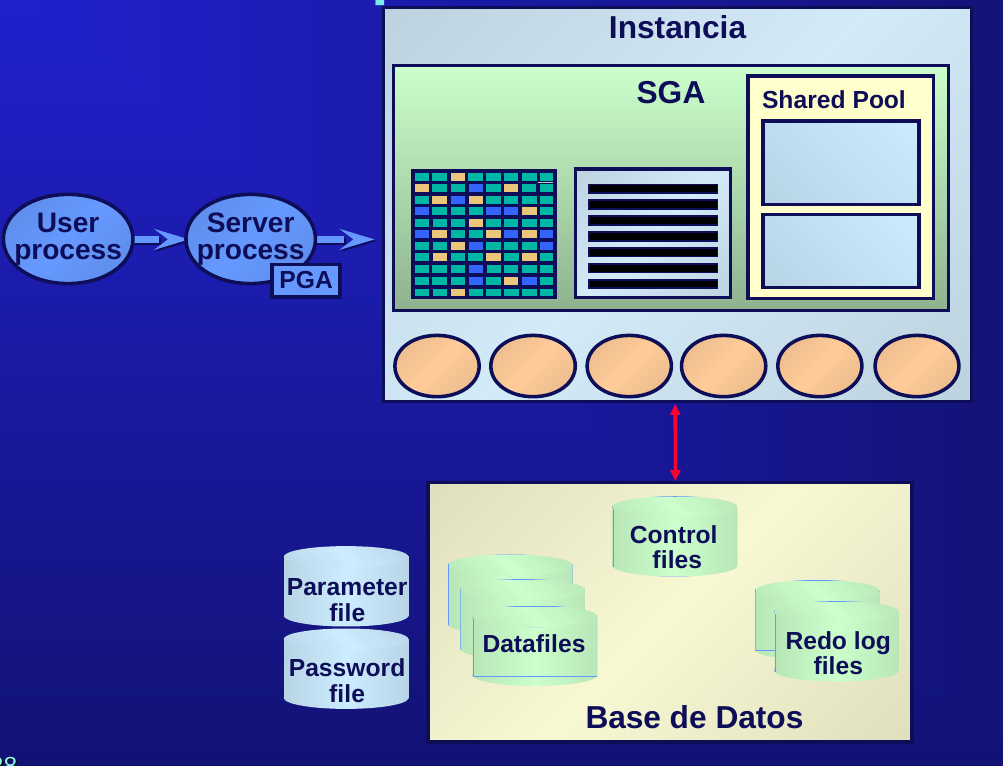
\includegraphics[scale=0.25]{img/p18.png}
\end{figure}
Normalmente esto lo hace el \textit{Asistente de Oracle}, pero ¿qué pasa si el asistente no funciona? El asistente simplemente traduce las opciones que le pasamos a órdenes que ejecuta en una línea de comandos.

Son necesarios unos prerequisitos mínimos para crear una base de datos:
\begin{itemize}
\item Una cuenta con privilegios autentificada de alguna de las siguientes formas:
\begin{itemize}
\item Por el sistema operativo.
\item Por el fichero de password.
\end{itemize}
\item Memoria para iniciar la instancia.
\item Espacio de disco suficiente para la base de datos planificada.
\end{itemize}

Con respecto a la planificación de la localización de los ficheros de la BD es necesario:
\begin{itemize}
\item Mantener al menos dos copias activas de los ficheros de control de la base de datos en diferentes discos. De hecho, la propia sentencia de creación de bases de datos no admite que solo le pases un fichero de control como parámetro. Sin embargo, si admite que los dos estén en el mismo disco.
\item Multiplexar los ficheros redo log y poner los miembros (archivos redo log) de los grupos en discos diferentes (duplicarlos). Un grupo es un conjunto de copias del mismo fichero redo log (miembro) en discos diferentes.
\item Separar los ficheros de datos cuyos datos:
\begin{itemize}
\item Puedan producir congestión en el almacenamiento secundario. Estos habría que distribuirlos en varios discos.
\item Presenten una duración permanente, es decir, hay que diferenciar entre temporales y permanentes.
\item Tengan características de administración diferentes.
\end{itemize}
\end{itemize}

\subsection{Localización del software Oracle}


\begin{figure}[H]
  \center
  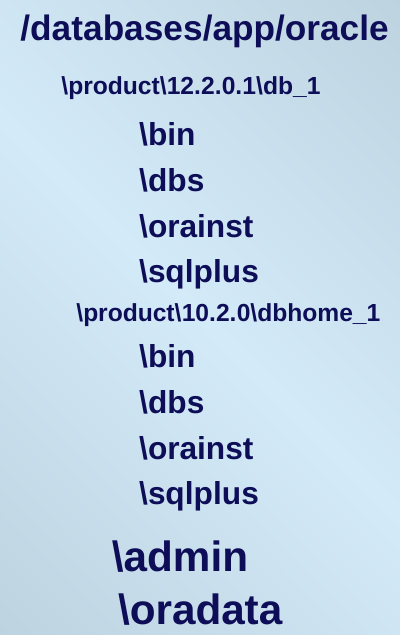
\includegraphics[scale=0.25]{img/p19.png}
\end{figure}

A la ruta \textit{/databases/app/oracle} se le llama \textit{ORACLE\_BASE} y a \textit{/product/11.2.0.1/db\_1} y \textit{/product/10.2.0/dbhome\_1} se les llama \textit{ORACLE\_HOME}.

\begin{figure}[H]
  \center
  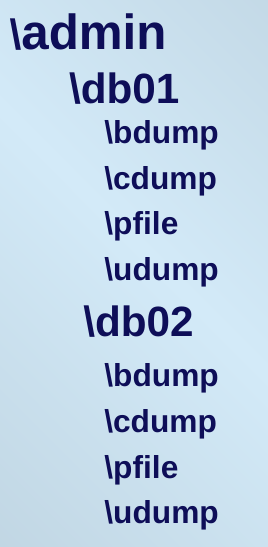
\includegraphics[scale=0.25]{img/p20.png}
\end{figure}

En \textit{admin} se mete toda la información relativa a la administración de Oracle. Hay una subcarpeta (\textit{db01} y \textit{db02}) para cada BD existente en el sistema. Esto implica que no podemos tener dos BD con el mismo nombre aún ejecutando cada una de ellas en versiones diferentes de Oracle.

La carpeta \textit{oradata} normalmente se encuentra distribuida en varios discos (como muestra la siguiente imagen) o incluso replicada en diferentes discos:
\begin{figure}[H]
  \center
  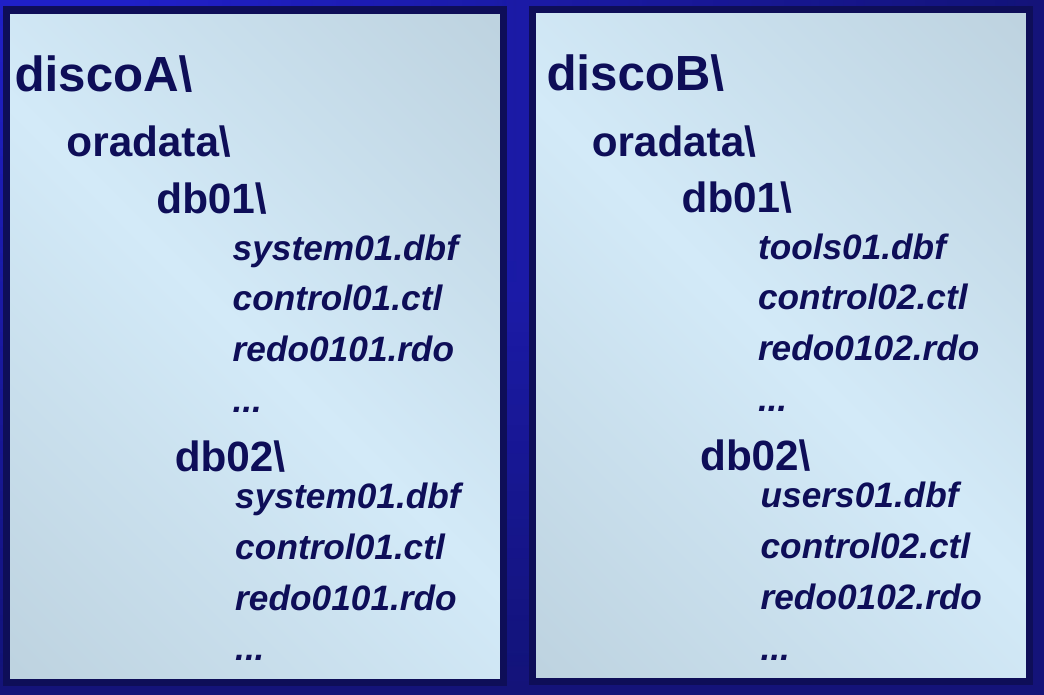
\includegraphics[scale=0.25]{img/p21.png}
\end{figure}
Esto nos permite hacer la multiplexación que se comentó antes de los redo logs y los control files.

\subsection{Creación manual}

Para la creación manual de una base de datos hay que seguir una serie de pasos. Antes de realizar estos pasos se recomienda clonar la máquina virtual para evitar romper la instalación sin querer.

\begin{itemize}
\item Determinar un nombre único para la instancia y la BD. Además hay que elegir un conjunto de caracteres.
\item Establecer las variables del sistema operativo:

\begin{lstlisting}[ language=bash,
                    deletekeywords={IDENTITY},
                    deletekeywords={[2]INT},
                    morekeywords={clustered},
                    framesep=8pt,
                    xleftmargin=40pt,
                    framexleftmargin=40pt,
                    frame=tb,
                    framerule=0pt ]
echo $ORACLE_BASE;
echo $ORACLE_HOME;
# PATH deberia tener incluida las rutas de oracle
echo $PATH;
# el sid es el identificador de la base de datos
# esta variable la consulta SQLPlus para saber a que BD 
# debe conectarse
echo $ORACLE_SID;
ORACLE_SID=prueba
export ORACLE_SID;
echo $ORACLE_SID;
\end{lstlisting}
La variable \textit{ORACLE\_SID} da problemas al crear una nueva base de datos porque cuando se intenta crear algo usando las herramientas de Oracle, estas consultarán esa variable para saber a qué BD modificar. Luego lo primero que se debe hacer es cambiar esa variable.
\item Crear un fichero de password (recomendado):
\begin{lstlisting}[ language=bash,
                    deletekeywords={IDENTITY},
                    deletekeywords={[2]INT},
                    morekeywords={orapwd},
                    framesep=8pt,
                    xleftmargin=40pt,
                    framexleftmargin=40pt,
                    frame=tb,
                    framerule=0pt]
# nos vamos al directorio donde se va a crear el fichero
# para poder verlo
cd $ORACLE_HOME/dbs
orapwd file=$ORACLE_HOME/dbs/orapwprueba entries=5
\end{lstlisting}
\item Preparar el fichero de parámetros. Esto es bastante lioso así que lo único que se va a hacer es copiar el fichero existente de la otra base de datos.
\begin{lstlisting}[ language=bash,
                    deletekeywords={IDENTITY},
                    deletekeywords={[2]INT},
                    morekeywords={mkdir, gedit,cp,df},
                    framesep=8pt,
                    xleftmargin=40pt,
                    framexleftmargin=40pt,
                    frame=tb,
                    framerule=0pt]
cp $ORACLE_BASE/admin/oradba/pfile/init.ora $ORACLE_HOME/dbs/initprueba.ora
# reemplazar todas las apariciones de 'oradba' por 'prueba'
gedit $ORACLE_HOME/dbs/initprueba.ora
# carpeta para los ficheros de control
mkdir $ORACLE_BASE/oradata/prueba
# carpeta para auditorias
mkdir $ORACLE_BASE/admin/prueba
mkdir $ORACLE_BASE/admin/prueba/adump
# comprobar espacio disponible para los pasos que quedan
cd $ORACLE_HOME/dbs
df -h
\end{lstlisting}
\item Iniciar la instancia.
\begin{lstlisting}[ language=bash,
                    deletekeywords={IDENTITY},
                    deletekeywords={[2]INT},
                    morekeywords={mkdir, gedit,cp,sqlplus},
                    framesep=8pt,
                    xleftmargin=40pt,
                    framexleftmargin=40pt,
                    frame=tb,
                    framerule=0pt]
sqlplus /nolog
connect sys as sysdba
STARTUP NOMOUNT PFILE='$ORACLE_HOME/dbs/initprueba.ora'
\end{lstlisting}
\item Crear la base de datos (se crea vacía, sin el diccionario de datos incluso).
\begin{lstlisting}[ language=sql,
                    deletekeywords={IDENTITY},
                    deletekeywords={[2]INT},
                    morekeywords={mkdir, gedit,cp,sqlplus},
                    framesep=8pt,
                    xleftmargin=5pt,
                    framexleftmargin=20pt,
                    frame=tb,
                    framerule=0pt]
create database prueba user sys identified by "ABD3,oradba"
user system identified by "ABD3,oradba"
logfile
group 1 ('/databases/app/oracle/oradata/prueba/redo01.log') size 10M,
group 2 ('/databases/app/oracle/oradata/prueba/redo02.log') size 10M,
group 3 ('/databases/app/oracle/oradata/prueba/redo03.log') size 10M
maxlogfiles 5
maxlogmembers 5
maxloghistory 1
maxdatafiles 100
maxinstances 1
character set us7ascii
national character set al16utf16
datafile '/databases/app/oracle/oradata/prueba/system01.dbf' size 350M reuse
extent management local
sysaux datafile '/databases/app/oracle/oradata/prueba/sysaux01.dbf' size 100M reuse 
default temporary tablespace temp
tempfile '/databases/app/oracle/oradata/prueba/temp01.dbf' size 20M reuse
undo tablespace undotbs1
datafile '/databases/app/oracle/oradata/prueba/undotbs1g01.dbf' size 50m reuse autoextend on next 5120k maxsize unlimited;
\end{lstlisting}
Ese archivo sql se puede bajar desde \url{https://decsai.ugr.es/~iblanco/scriptBD.sql}. Para ejecutarlo:
\begin{lstlisting}[ language=bash,
                    deletekeywords={IDENTITY},
                    deletekeywords={[2]INT},
                    morekeywords={mkdir, gedit,cp,sqlplus},
                    framesep=8pt,
                    xleftmargin=40pt,
                    framexleftmargin=40pt,
                    frame=tb,
                    framerule=0pt]
@/home/oracle/Descargas/scriptBD.sql
\end{lstlisting}
\item Ejecutar los "scripts" para generar el diccionario de datos, los paquetes almacenados y demás procesos de poscreación. posteriores.

Ver siguiente sección.
\end{itemize}

\subsection{Creación de vistas de diccionario y paquetes}

Lo primero que hay que hacer es crear las denominadas \textit{tablas base}. Son tablas muy normalizadas, es decir, la información en ellas está muy dividida para que no haya que mantenerlas. A continuación se crean las \textit{vistas del diccionario de datos}, que consultan las tablas base para mostrar la información relativa a un usario, etc. Para generarlas: 
\begin{lstlisting}[ language=bash,
                    deletekeywords={IDENTITY},
                    deletekeywords={[2]INT},
                    morekeywords={mkdir, gedit,cp,SQLPlus},
                    framesep=8pt,
                    xleftmargin=40pt,
                    framexleftmargin=40pt,
                    frame=tb,
                    framerule=0pt]
# crea las vistas de diccionario habitualmente usadas
SQLPlus> @$ORACLE_BASE/product/12.2.0.1/db_1/rdbms/admin/catalog.sql
# ejecuta todos los scripts para ejecutar PL/SQL en el servidor
SQLPlus> @$ORACLE_BASE/product/12.2.0.1/db_1/rdbms/admin/catproc.sql
\end{lstlisting}
Estos dos scripts necesitan bastante tiempo para terminar de ejecutarse, asi que ten paciencia! Una vez que terminen, ya se habrá creado la base de datos.

\subsection{Vistas del diccionario de datos}

\begin{figure}[H]
  \center
  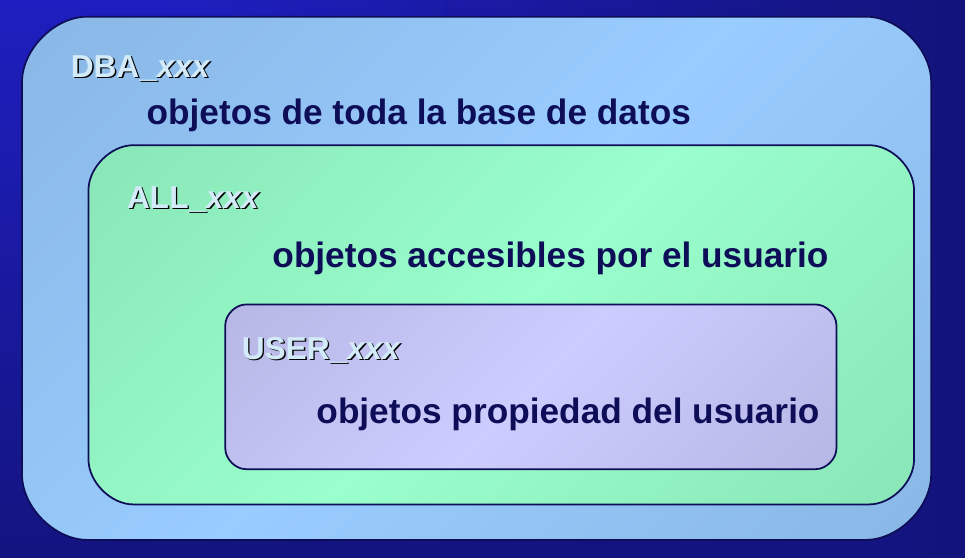
\includegraphics[scale=0.25]{img/p23.png}
  \caption{Esquema del diccionario de datos}
\end{figure}
\begin{figure}[H]
  \center
  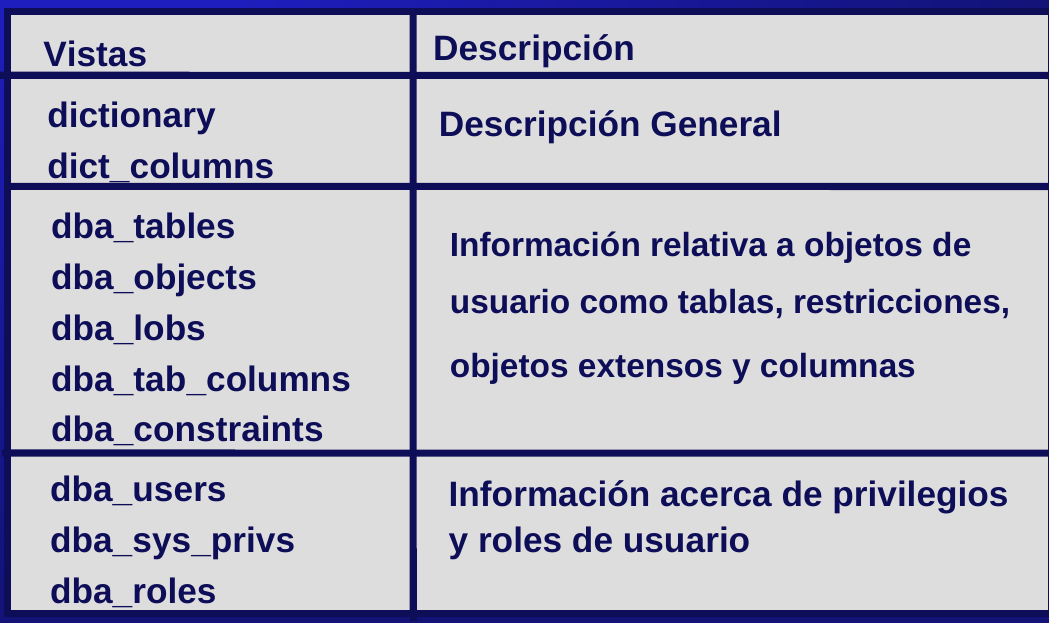
\includegraphics[scale=0.2]{img/p24.png}
  \caption{Ejemplos de vistos y categorías}
  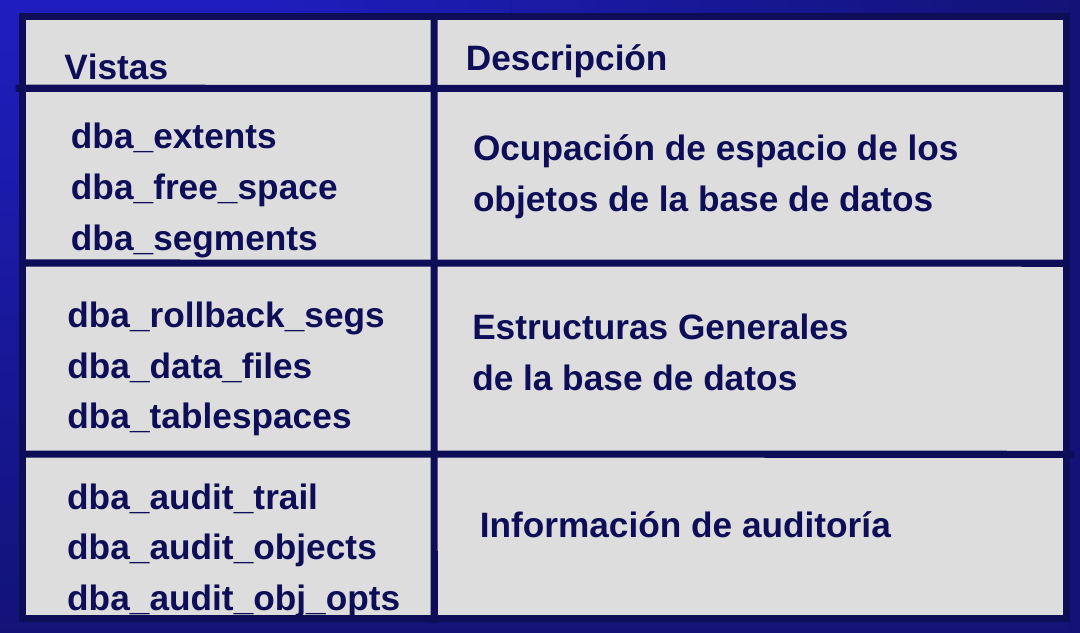
\includegraphics[scale=0.2]{img/p25.png}
  \caption{Más ejemplos}
\end{figure}